\documentclass[tikz,border=5pt]{standalone}
\usepackage{tikz}
\usetikzlibrary{arrows.meta,matrix,cd}

\begin{document}
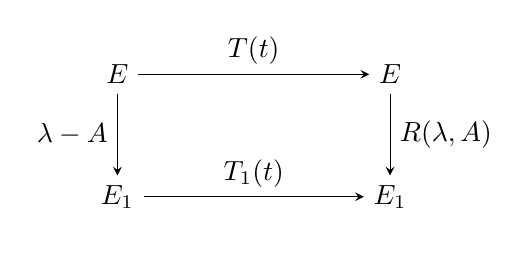
\begin{tikzpicture}[
    >=stealth,
    every node/.style={transform shape}
]
    % Matrix mit optimiertem Spacing
    \matrix (m) [
        matrix of math nodes,
        row sep=3em,    
        column sep=4em,
        nodes={anchor=center}
    ] {
        E    & & E \\
        E_{1}  & & E_{1} \\
    };
    % Pfeile als Pfad mit verbesserter Positionierung
    \path[->]
        (m-1-1) edge node[above] {$T(t)$} (m-1-3)
        (m-2-1) edge node[above] {$T_{1}(t)$} (m-2-3)
        (m-1-1) edge node[left] {$\lambda-A$} (m-2-1)
        (m-1-3) edge node[right] {$R(\lambda,A)$} (m-2-3);
    
\end{tikzpicture}\end{document}
